%FOR PDFLATEX USE ONLY
\documentclass[a4paper,12pt]{article}

\usepackage{amssymb,amsmath}

\usepackage[margin=2cm]{geometry}
\usepackage[unicode]{hyperref}
\usepackage[pdftex]{graphicx}
\usepackage{cmlgc}

\usepackage{array}

\usepackage{wrapfig}
\usepackage{array}
\usepackage{lipsum}
\usepackage{esvect}
\usepackage{hyperref}

\usepackage{subfig}
\usepackage{calc}
\usepackage{pgfplots,tikz,circuitikz}
\usepackage{pgfplotstable}
\usepackage{tkz-euclide}

\usepackage{centernot}
\usepackage{cancel}

\usepackage{mathtext}
\usepackage[T1,T2a]{fontenc}
\usepackage[utf8]{inputenc}
\usepackage[english, bulgarian, russian]{babel}
\usepackage{tikz}
\usepackage{pgfplots}
\usepackage[export]{adjustbox}
\usepackage[left=2cm,right=2cm,
    top=2cm,bottom=2cm,bindingoffset=0cm]{geometry}
\usepackage{indentfirst}
\usepackage{braket}

\begin{document}

\begin{center}
  \LARGE{Работа 1.2.1}\\[0.2cm]
  \LARGE{Определение скорости полета пули при помощи баллистического маятника}\\[0.2cm]
  \large{Малиновский Владимир}\\[0.2cm]
  \normalsize{\texttt{galqiwi@galqiwi.ru}}
\end{center}

\textbf{Цель работы:} определить скорость полета пули, применяя законы созранения и используя баллистические маятники.

\textbf{В работе используются:} духовое ружье на штативе, осветитель, оптическая система для измерения отклонений маятника, измерительная линейка, пули и весы для их взвенивания, а также баллистические маятники.

\section{Метод баллистического маятника, совершающего поступательное движение}

\begin{figure}[h]
\begin{center}$
\begin{array}{cc}
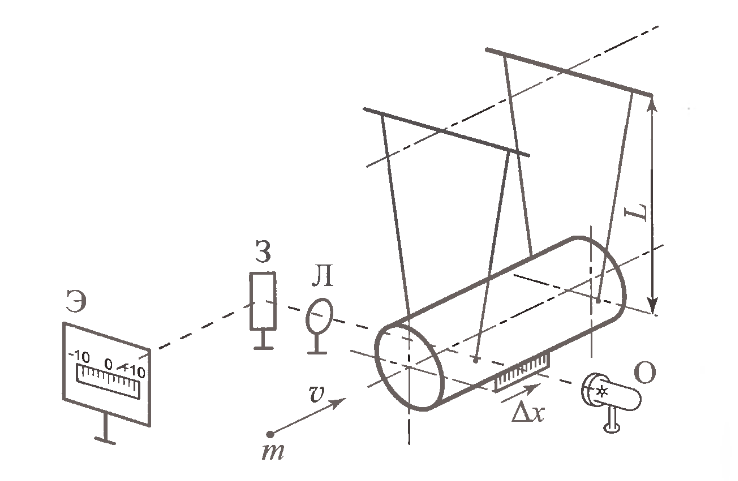
\includegraphics[width=0.45\textwidth]{prop-1.png}&
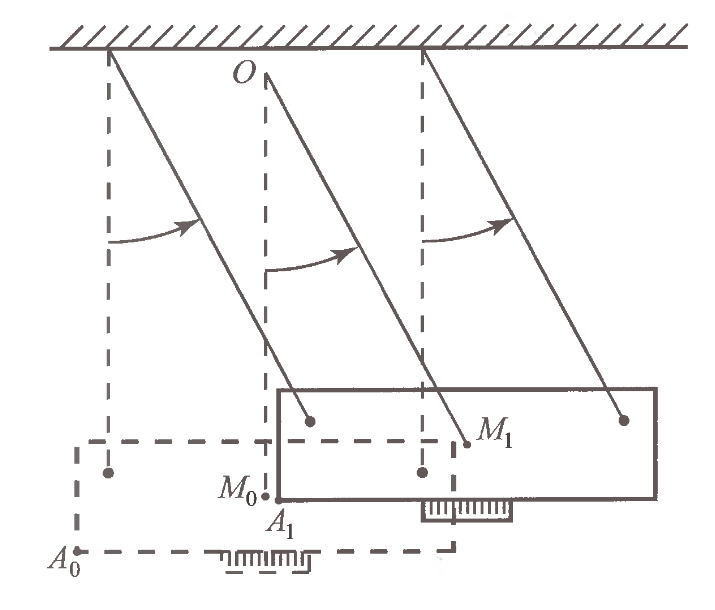
\includegraphics[width=0.45\textwidth]{prop-2.png}\\
\text{рис. 1, схема установки} & \text{рис. 2, поведение баллистического маятника}\\
&\text{при попадании в него пули.}
\end{array}$
\end{center}
\end{figure}
В этой части используется установка, изображенная на рис. 1. Если масса маятника равна $M$, то скорость системы маятник-пуля сразу после попадания маятника равна
\begin{equation}
v_0 = \frac{m}{M + m}v.
\end{equation}
У маятника угловая скорость $\omega = \sqrt{g/L}$. Если у него амплитуда $A$, то верно, что
\begin{equation}
A \omega = v_0.
\end{equation}
Из этого скорость выражается, как
\begin{equation}
v = \sqrt{\frac{g}{L}}\frac{M+m}{m}A.
\end{equation}
\newpage
\subsection{Результаты и обработка}

Массы пулек:
\begin{figure}[h]
\begin{center}$
\begin{array}{|c|c|c|c|c|c|c|c|c|c|c|}
\hline
N & 1 & 2 & 3 & 4 & 5 & 6 & 7 & 8 & 9 & 10 \\
\hline
m\text{, г} & 0.5128 & 0.5110 & 0.5120 & 0.5160 & 0.5090 & 0.5174 & 0.5039 & 0.5172 & 0.5083 & 0.5000 \\
\hline
\end{array}$
\end{center}
\caption*{$\Delta m = 0.001\text{г}$}
\end{figure}

$L = (2208\pm10)$ мм, $M=(2900\pm5)$ г.

Амплитуды и соответствующие скорости:

\begin{figure}[h]
\begin{center}$
\begin{array}{|c|c|}
\hline
A\text{, мм} & v\text{, м/c} \\
\hline
12.2\pm0.2 & 145\pm3 \\
\hline
12.2\pm0.2 & 146\pm3 \\
\hline
12.2\pm0.2 & 146\pm3 \\
\hline
12.2\pm0.2 & 145\pm3 \\
\hline
\end{array}$
\end{center}
\end{figure}

Усредняя, получаем $<v>=(146\pm3)\text{, м/c}$.

\section{Метод крутильного баллистического маятника}
В этом методе используется установка, изображенная на рис. 3.
\begin{figure}[h]
\begin{center}$
\begin{array}{c}
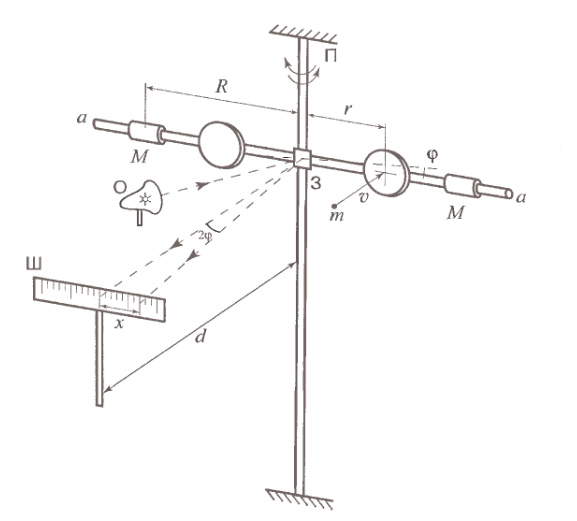
\includegraphics[width=0.73\textwidth]{rot.png}\\
\text{рис. 3, крутильный баллистический маятник.}
\end{array}$
\end{center}
\end{figure}
\newpage
Сразу после попадания пули в мишень, система пуля-мишень будет двигаться с угловой скоростью $\Omega$ такой, что
\begin{equation}
m v r = I \Omega,
\end{equation}
где $I$ -- момент инерции систему пуля-мишень.\\
Если $k$ -- модуль кручения проволоки, то из закона сохранения энергии следует, что
\begin{equation}
k \frac{\varphi^2}{2} = I \frac{\Omega^2}{2},
\end{equation}
где $\varphi$ -- амплитуда колебаний маятника после выстрела.
Из уравнений (4) и (5) можно найти скорость $v$ по амплитуде $\varphi$.
\begin{equation}
v = \varphi \frac{\sqrt{kI}}{mr}.
\end{equation}

Есть два метода расчета $\varphi$ -- простой и сложный.
\begin{equation}
\varphi_s = \frac{|x_0 - x_1|}{d}, \varphi_h = |atan(\frac{x_0}{d}) - atan(\frac{x_1}{d})| / 2.
\end{equation}

Если система колебается с периодом $T$, то верно, что ее момент инерции равен:

\begin{equation}
I = \frac{k}{4\pi^2}T^2.
\end{equation}

Если грузов на маятнике нет, то момент инерции системы обозначим за $I_0$. Если есть, то он равен

\begin{equation}
I = I_0 + 2 \Delta I + 2 M R^2,
\end{equation}

Где $M$ -- масса одного груза, a $\Delta I$ -- момент инерции груза относительно вертикальной оси, проходящей через его центр.

\subsection{Результаты и обработка}

Данные для момента инерции

\begin{figure}[h]
\begin{center}$
\begin{array}{|c|c|c|c|c|c|c|c|}
\hline
R\text{, мм} & R^2\text{, м$^2$} & T_5\text{, c} & T_5\text{, c} & T\text{, c} & T^2\text{, c$^2$} & \Delta T\text{, c} & \Delta T^2\text{, c$^2$}\\
\hline
0^* & 0^* & 38.66 & 38.60 & 7.726 & 59.7 & 0.2 & 0.6\\
\hline
329 & 0.108 & 56.03 & 56.54 & 11.26 & 126.7 & 0.2 & 0.9\\
\hline
303 & 0.0918 & 53.68 & 54.22 & 10.79 & 116.4 & 0.2 & 0.9\\
\hline
273 & 0.0745 & 51.34 & 51.56 & 10.29 & 105.9 & 0.2 & 0.8\\
\hline
\end{array}$
\end{center}
\caption{*без учета момента инерции грузов}
\end{figure}

Из линейности графика на рис. 4, следует, что $\Delta I << I$, то есть собственный момент инерции грузов меньше погрешности измерения момента инерции.\\
Из МНК следует, что
\begin{equation}
\begin{cases}
\displaystyle \frac{4\pi^2}{k}I_0 =(59.68\pm0.13)\text{с}^2 \\
\displaystyle \frac{4\pi^2}{k}2M = (620\pm2)\text{с}^2/\text{м}^2.\\
\end{cases}
\end{equation}

\newpage

\begin{figure}[h]
\begin{center}$
\begin{array}{c}
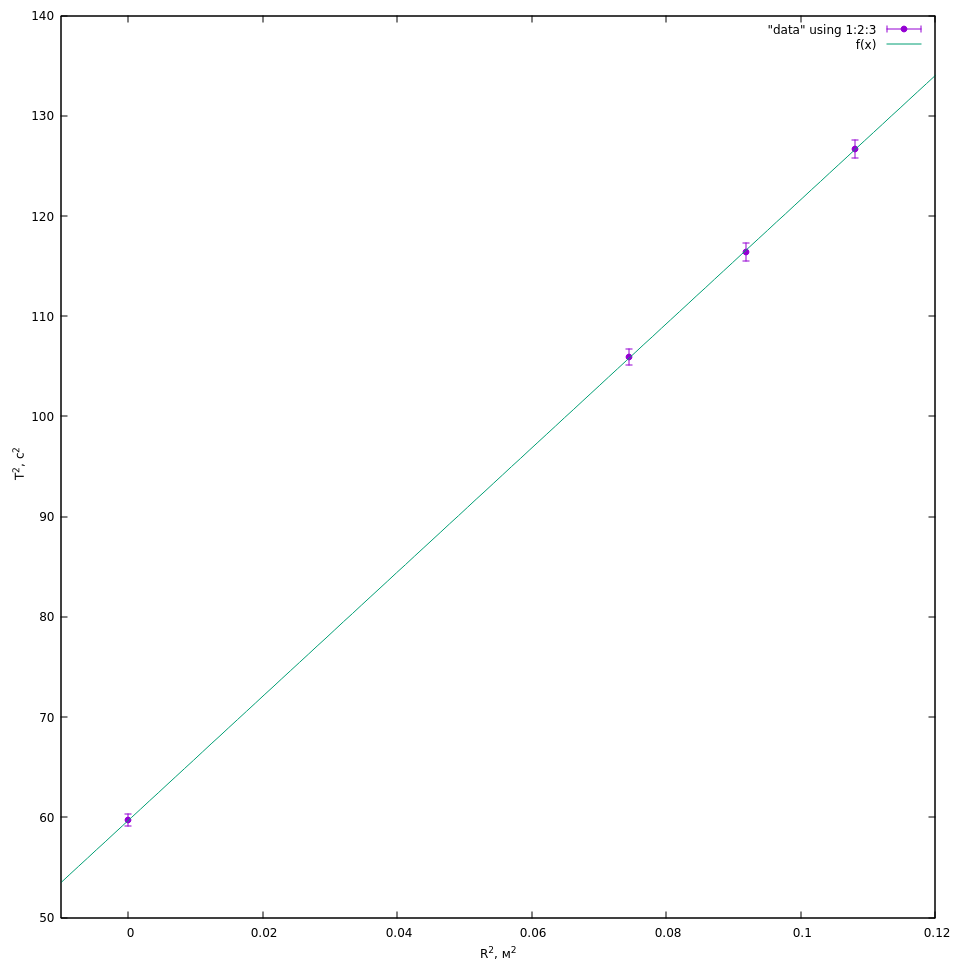
\includegraphics[width=1\textwidth]{inertia.png}\\
\text{рис. 4, график зависимости $T^2$ от $R^2$.}\\
\end{array}$
\end{center}
\end{figure}

Из уравнений (10) можно найти $k = (0.0929\pm0.0003) \text{ кг$\cdot$м$^2/$c$^2$}$.

\begin{equation}
v = \varphi \frac{\sqrt{kI}}{mr} = \varphi \frac{kT}{2\pi mr}.
\end{equation}

\newpage
Амплитуды и скорости:

\begin{figure}[h]
\begin{center}$
\begin{array}{|c|c|c|c|c|c|c|c|c|}
\hline
x_0\text{, см}&\Delta x_0\text{, см}& x_1\text{, см}& m\text{, г}& T\text{, с}& \varphi_s & \varphi_h & v_s\text{, м$/$с} & v_h\text{, м$/$с}\\
\hline
7.2& 0.4& -0.1& 0.5090& 7.73& 0.113\pm0.008& 0.114\pm0.008& 126\pm10& 127\pm10\\
\hline
7.2& 0.4& -0.1& 0.5174& 7.73& 0.113\pm0.008& 0.114\pm0.008& 124\pm10& 125\pm10\\
\hline
4.9& 0.3& -0.4& 0.5039& 11.26& 0.083\pm0.007& 0.083\pm0.007& 136\pm12& 136\pm12\\
\hline
6.6& 0.2& 0.2& 0.5172& 10.79& 0.100\pm0.005& 0.101\pm0.006& 153\pm9& 154\pm10\\
\hline
7.5& 0.1& 1.0& 0.5083& 10.29& 0.102\pm0.004& 0.103\pm0.005& 151\pm7& 152\pm8\\
\hline
7.5& 0.2& 1.3& 0.5000& 10.29& 0.097\pm0.005& 0.098\pm0.006& 146\pm9& 148\pm10\\
\hline
\end{array}$
\end{center}
\caption{$\Delta x_1 = 0.05\text{ см}$, $d = (32\pm0.5)\text{ см}$.}
\end{figure}

Во 2 методе получается значение
$<v> = (140 \pm 11)\text{м/c}$.

При том, что $<v_s> = (139 \pm 11)\text{м/c}$.

В моей работе значения скоростей, полученные двумя разными методами, сходятся:
\begin{equation}
v_0 = (146 \pm 3)\text{м/c}, v_1 = (140 \pm 11)\text{м/c}.
\end{equation}

При этом я слышал, что у других людей на 2 установке получались значения скорости больше, чем на первой. Виной этому точно не неучет собственного момента инерции грузов в лабнике, поскольку во второй части у меня получилось, что он слишком мал. Также это не может происходить из-за приближения тангенса линейной функцией во 2 пункте, у меня отклонение финального ответа при линейном приближении получилось меньше процента от честного. Данный эффект может происходить из-за:
\begin{enumerate}
\item \text{Трения о воздух}
\item \text{Того, что по-настоящему этого эффекта нет -- все говорят, что он есть, но,}\\\text{честно промерив, его никто не получил, возможно, даже,}\\\text{некоторые студенты подогнали свои значения так, что этот эффект}\\\text{специально начал проявляться, что укрепило миф.}
\item \text{какой-то другой эффект, который не пришел мне в голову.}
\end{enumerate}
Рассмотрим трение о воздух. Диаметр пули равен $4.5\text{ мм}$, расстояние до цели порядка $80\text{ см}$ на различных установках, скорость пули порядка $140\text{ м$/$с}$. Посмотрим, насколько пуля замедлится.\\
Если брать квадратичную зависимость ($F=C_f\displaystyle \frac{\rho v^2}{2}S$) силы трения от скорости, то на пулю действует сила в $153\text{ мН}$, если считать пулю цилиндром. При массе в $0.5\text{ г}$, пуля успеет замедлиться на $1.7\text{ м/c}$ за это время. Поскольку порядок вариации расстояния от конца ствола до мишени -- $10\text{ см}$, что в 8 раз меньнше, получим вариацию в $0.2\text{ м/c}$ по скорости, что много меньше погрешности. Это не трение.
\section{Вывод}
Я получил значение скорости пули двумя методами -- методом баллистического маятника и методом крутильного маятника. Значения скорости совпали с точностью до погрешности. Физического объяснения того, что у других студентов получаются разные значения я не нашел, хотя рассмотрел три варианта: неучет момента инерции грузов, неучет нелинейности тангенса при расчете амплитуды отклонения и неучет силы трения о воздух.

\end{document}








\lipsum[1-4]
\begin{wrapfigure}{R}{5cm}
\centering
\includegraphics[width=0.20\textwidth]{rd.png}
\caption{1}
\end{wrapfigure}
\lipsum[1-6]


\begin{figure}[h]
\begin{center}$
\begin{array}{cccc}
\includegraphics[width=0.20\textwidth]{rd.png}&
\includegraphics[width=0.20\textwidth]{rd.png}&
\includegraphics[width=0.20\textwidth]{rd.png}&
\includegraphics[width=0.20\textwidth]{rd.png}\\
(1) & (2) & (3) & (4)
\end{array}$
\end{center}
\end{figure}
